%\VignetteIndexEntry{penalized}

\documentclass[a4paper]{article}
\usepackage{natbib}
\bibliographystyle{chicago}

\newcommand{\Robject}[1]{{\texttt{#1}}}
\newcommand{\Rfunction}[1]{{\texttt{#1}}}
\newcommand{\Rpackage}[1]{{\textit{#1}}}
\newcommand{\Rclass}[1]{{\textit{#1}}}
\newcommand{\Rfunarg}[1]{{\textit{#1}}}

\sloppy

\title{L1 and L2 Penalized Regression Models}

\author{Jelle Goeman}

\usepackage{c:/R/R-2.6.0dev/share/texmf/Sweave}
\begin{document}

\maketitle \tableofcontents \newpage

\section{Introduction}

This short note explains the use of the \Rpackage{penalized} package. The package is designed for penalized estimation in generalized linear models.

The supported models at this moment are linear regression, logistic regression and the Cox proportional hazards model, but others are likely to be included in the future. As to penalties, the package allows an L1 absolute value (``lasso'') penalty \citep{Tibshirani1996, Tibshirani1997}, an L2 quadratic (``ridge'') penalty \citep{Hoerl1970, Cessie1992, Verweij1994}, or a combination of the two \citep[the ``naive elastic net'' of][]{Zou2005}. The package also includes facilities for likelihood cross-validation and for optimization of the tuning parameter.

L1 and L2 penalized estimation methods shrink the estimates of the regression coefficients towards zero relative to the maximum likelihood estimates. The purpose of this shrinkage is to prevent overfit arising due to either collinearity of the covariates or high-dimensionality. Although both methods are shrinkage methods, the effects of L1 and L2 penalization are quite different in practice. Applying an L2 penalty tends to result in all small but non-zero regression coefficients, whereas applying an L1 penalty tends to result in many regression coefficients shrunk exactly to zero and a few other regression coefficients with comparatively little shrinkage. Combining L1 and L2 penalties tends to give a result in between, with fewer regression coefficients set to zero than in a pure L1 setting, and more shrinkage of the other coefficients. The amount of shrinkage is determined by tuning parameters $\lambda_1$ and $\lambda_2$. A value of zero always means no shrinkage (= maximum likelihood estimation) and a value of infinity means infinite shrinkage (= setting all regression coefficients to zero). For more details about the methods, please refer to the above-mentioned papers.

It is important to note that shrinkage methods are generally not invariant to the relative scaling of the covariates. Before fitting a model, it is prudent to consider if the covariates already have a natural scaling relative to each other or whether they should be standardized.

The main algorithm for L1 penalized estimation that used in this package will be documented in a forthcoming paper. It has been combined with ideas from \cite{Eilers2001} and \cite{Houwelingen2006} for efficient L2 penalized estimation.


\section{Penalized likelihood estimation}

The basic function of the package is the \Rfunction{penalized} function, which performs penalized estimation for fixed values of $\lambda_1$ and $\lambda_2$. Its syntax has been loosely modeled on that of the functions \Rfunction{glm} (package \Rpackage{stats}) and \Rfunction{coxph} (package \Rpackage{survival}), but it is slightly more flexible. Two main input types are allowed: one using \Rclass{formula} objects, one using matrices.

\subsection{the nki70 data}

As example data we use the 70 gene signature of \cite{Veer2002} in the gene expression data set of \cite{Vijver2002}.

\begin{Schunk}
\begin{Sinput}
> library(penalized)
> data(nki70)
\end{Sinput}
\end{Schunk}

This loads a \Rclass{data.frame} with 144 breast cancer patients and 77 covariates. The first two covariates indicate the survival time and event status (time is in months), the next five are clinical covariates (diameter of the tumor, lymph node status, estrogen receptor status, grade of the tumor and age of the patients), and the other 70 are gene expression measurements of the 70 molecular markers.

\subsection{the penalized function}

To fit a model to predict survival (\Robject{Surv(time,event)}) with the two markers ``DIAPH3'' and ``NUSAP1'' at $\lambda_1 = 0$ and $\lambda_2 = 1$, we can say (all are equivalent)

\begin{Schunk}
\begin{Sinput}
> fit <- penalized(Surv(time, event), ~DIAPH3 + NUSAP1, data = nki70, 
      lambda2 = 1)
> fit <- penalized(Surv(time, event), nki70[, 10:11], data = nki70, 
      lambda2 = 1)
> fit <- penalized(Surv(time, event) ~ DIAPH3 + NUSAP1, data = nki70, 
      lambda2 = 1)
\end{Sinput}
\end{Schunk}

The covariates may be specified in the second function argument (\Rfunarg{penalized}) as a \Rclass{formula} object with an open left hand side, as in the first line. Alternatively, they may be specified as a matrix, as in the second line. If, as here, they are supplied as a \Rclass{data.frame}, they are coerced to a matrix.

For consistency with \Rfunction{glm} and \Rfunction{coxph} the third option is also allowed, in which the covariates are included in the first function argument.

Use \Rfunction{attach} to avoid specifying the \Rfunarg{data} argument every time.

\begin{Schunk}
\begin{Sinput}
> attach(nki70)
\end{Sinput}
\end{Schunk}

\subsection{choice of lambda}

It is difficult to say in advance which value of \Rfunarg{lambda1} or \Rfunarg{lambda2} to use. The \Rpackage{penalized} package offers ways of finding optimal values using cross-validation. This is explained in Section \ref{cv}

Note that for small values of \Rfunarg{lambda1} or \Rfunarg{lambda2} the algorithm be very slow, may fail to converge or may run into numerical problems, especially in high-dimensional data. When this happens, increase the value of \Rfunarg{lambda1} or \Rfunarg{lambda2}.


\subsection{standardization}

If the covariates are not naturally on the same scale, it is advisable to standardize them. The function argument \Rfunarg{standardize} (default: \Robject{FALSE}) standardizes the covariates to unit second central moment before applying penalization. This standardization makes sure that each covariate is affected more or less equally by the penalization.

The fitted regression coefficients that the function returns have been scaled back and correspond to the original scale of the covariates.


\subsection{penfit objects}

The penalized function returns a \Rclass{penfit} object, from which useful information can be extracted. For example, to extract regression coefficients, (martingale) residuals, individual relative risks and baseline hazard, write

\begin{Schunk}
\begin{Sinput}
> coefficients(fit)
\end{Sinput}
\begin{Soutput}
      DIAPH3       NUSAP1 
-0.003347245  1.610876235 
\end{Soutput}
\begin{Sinput}
> residuals(fit)[1:10]
\end{Sinput}
\begin{Soutput}
       125        127        128        129        130        132        134 
-0.1299336  0.7104811 -0.3517060 -0.2083512 -0.4264021 -0.3621108  0.7464918 
       135        136        137 
-0.6172103  0.7367359 -0.4470460 
\end{Soutput}
\begin{Sinput}
> fitted.values(fit)[1:10]
\end{Sinput}
\begin{Soutput}
      125       127       128       129       130       132       134       135 
0.4023261 1.0605204 0.8671254 0.6451380 1.3203100 1.1783128 0.7849620 1.3615191 
      136       137 
1.2242175 0.5909803 
\end{Soutput}
\begin{Sinput}
> basehaz(fit)
\end{Sinput}
\begin{Soutput}
A "breslow" object with 1 survival curve and 50 time points.
\end{Soutput}
\end{Schunk}

See \Robject{help(penfit)} for more information on \Rclass{penfit} objects and Section \ref{breslow} on \Rclass{breslow} objects.


\subsection{unpenalized covariates}

In some situations it is desirable that not all covariates are subject to a penalty. Any additional covariates that should be included in the model without being penalized can be specified separately. using the third function argument (\Rfunarg{unpenalized}). For example

\begin{Schunk}
\begin{Sinput}
> fit <- penalized(Surv(time, event), nki70[, 8:77], ~ER, lambda2 = 1)
\end{Sinput}
\end{Schunk}

This adds estrogen receptor status as an unpenalized covariate.

In linear and logistic regression the intercept is by default never penalized.

In rare cases  each covariate may have to penalized in a different way, or some covariates have to be given an L2 penalty and others an L1 penalty. In those cases, the arguments \Rfunarg{lambda1} and \Rfunarg{lambda2} may be supplied as vectors of the same length as the number of covariates in the function argument \Rfunarg{penalized}.


\subsection{factors}

If some of the factors included in the \Rclass{formula} object \Rfunarg{penalized} are of type \Rclass{factor}, these are automatically made into dummy variables, as in \Rfunction{glm} and \Rfunction{coxph}, but in a special way that is more appropriate for penalized regression.

Unordered factors are turned into as many dummy variables as the factor has levels. This ensures a symmetric treatment of all levels and guarantees that the fit does not depend on the ordering of the levels. See \Robject{help(contr.none)} for details.

Ordered factors are turned into dummy variables that code for the difference between successive levels (one dummy less than the number of levels). L2 penalization on such factors therefore leads to small successive differences; L1 penalization leads to ranges of successive levels with identical effects. See \Robject{help(contr.diff)} for details.

To override the automatic choice of contrasts, use \Rfunction{C} (package \Rpackage{stats}).


\subsection{fitting in steps}

In some cases it may be interesting to visualize the effect of changing the tuning parameter \Rfunarg{lambda1} or \Rfunarg{lambda2} on the values of the fitted regression coefficients. This can be done using the function argument \Rfunarg{steps} in combination with the \Rfunction{plotpath} function. At this moment, this functionality is only available for visualizing the effect of \Rfunarg{lambda1}.

When using the \Rfunarg{steps} argument, the function starts fitting the model at the maximal value of $\lambda_1$, that is the smallest value that shrinks all regression coefficients to zero. From that value it continues fitting the model for \Rfunarg{steps} successively decreasing values of $\lambda_1$ until the specified value of \Rfunarg{lambda1} is reached.

If the argument \Rfunarg{steps} is supplied to \Rfunction{penalized}, the function returns a \Rclass{list} of \Rclass{penfit} objects. These can be accessed individually or their coefficients can be plotted using \Rfunction{plotpath}.

\begin{Schunk}
\begin{Sinput}
> fit <- penalized(Surv(time, event), nki70[, 8:77], lambda1 = 1, 
      steps = 50, trace = FALSE)
> plotpath(fit, log = "x")
\end{Sinput}
\end{Schunk}

\begin{figure}
\begin{Schunk}
\begin{Sinput}
> plotpath(fit, log = "x")
\end{Sinput}
\end{Schunk}
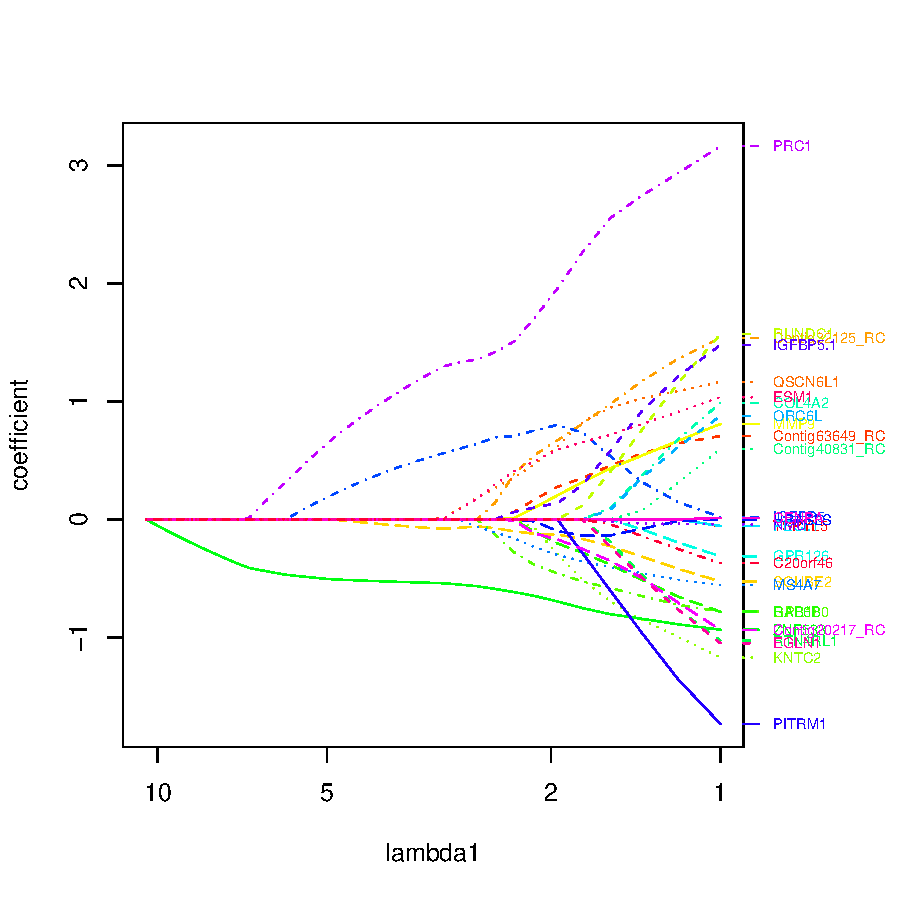
\includegraphics{penalized-stepsplot}
\end{figure}


\section{Cross-validation and optimization} \label{cv}

Cross-validation can be used to assess the predictive quality of the penalized prediction model or to compare the predictive ability of different values of the tuning parameter.

The \Rpackage{penalized} package uses likelihood cross-validation for all models. Likelihood cross-validation has some advantages over other optimization criteria: it tends to be a continuous function of the tuning parameter; it can be defined in a general way for almost any model, and it does not require calculation the effective dimension of a model, which is problematic in L1 penalized models. For the Cox proportional hazards model, the package uses cross-validated log partial likelihood \citep{Verweij1993}, which is a natural extension of the cross-validated log likelihood to the Cox model.

Five functions are available for calculating the cross-validated log likelihood and for optimizing the cross-validated log likelihood with respect to the tuning parameters. They have largely the same arguments. See \Robject{help(cvl)} for an overview.


\subsection{cross-validation}

The function \Rfunction{cvl} calculates the cross-validated log likelihood for fixed values of $\lambda_1$ and $\lambda_2$.

It accepts the same arguments as \Rfunction{penalized} (except \Rfunarg{steps}: see \Rfunction{profL1} below) as well as the \Rfunarg{fold} argument. This will usually be a single number $k$ to indicate $k$-fold cross-validation. In that case, the allocation of the subjects to the folds is random. Alternatively, the precise allocation of the subjects into the folds can be specified by giving \Rfunarg{fold} as a vector of the length of the number of subjects with values form 1 to $k$, each indicating the fold allocation of the corresponding subject. The default is to do leave-one-out cross-validation. 

The function \Rfunction{cvl} returns a names \Rclass{list} with four elements:
\begin{description}
\item[\Robject{cvl}] the cross-validated log likelihood.
\item[\Robject{fold}] the fold allocation used; this may serve as input to a next call to \Rfunction{cvl} to ensure comparability.
\item[\Robject{predictions}] the predictions made on each left-out subject. The format depends on the model used. In logistic regression this is just a vector of probabilities. In the Cox model this is a collection of predicted survival curves (a \Rclass{breslow} object). In the linear model this is a collection of predicted means and predicted standard deviations (the latter are the maximum penalized likelihood estimates of $\sigma^2$).
\item[\Robject{fullfit}] the fit on the full data (a \Rclass{penfit} object)
\end{description}

\begin{Schunk}
\begin{Sinput}
> fit <- cvl(Surv(time, event), nki70[, 8:77], lambda1 = 1, fold = 10)
\end{Sinput}
\end{Schunk}
\begin{Schunk}
\begin{Sinput}
> fit$cvl
\end{Sinput}
\begin{Soutput}
[1] -260.5181
\end{Soutput}
\begin{Sinput}
> fit$fullfit
\end{Sinput}
\begin{Soutput}
Penalized cox regression object
70 regression coefficients of which 28 are non-zero

Loglikelihood =	 -214.92 
L1 penalty =	 24.29771 	at lambda1 =  1 
\end{Soutput}
\end{Schunk}
\begin{Schunk}
\begin{Sinput}
> fit <- cvl(Surv(time, event), nki70[, 8:77], lambda1 = 2, fold = fit$fold)
\end{Sinput}
\end{Schunk}


\subsection{breslow objects} \label{breslow}

The \Rclass{breslow} class is defined in the \Rpackage{penalized} package to store estimated survival curves. They are used for the predictions in cross-validation and for the baseline hazard in the \Rfunction{penalized} function. See \Robject{help(breslow}) for details.

\begin{Schunk}
\begin{Sinput}
> fit$predictions
\end{Sinput}
\begin{Soutput}
A "breslow" object with 144 survival curves and 51 time points.
\end{Soutput}
\begin{Sinput}
> time(fit$predictions)
\end{Sinput}
\begin{Soutput}
 [1]  0.0000000  0.3531828  0.6488706  0.9363276  0.9609856  1.2101300
 [7]  1.3880903  1.5003422  1.6098563  1.6125941  1.7166324  1.7330595
[13]  1.9466119  1.9657769  1.9739904  2.2231348  2.2970568  2.3353867
[19]  2.3408624  2.6146475  2.6803559  2.6967830  2.8117728  2.8528405
[25]  3.1211499  3.2197125  3.4195756  3.4387406  3.6550308  3.9151266
[31]  4.2190281  4.4462697  4.6214921  4.6625599  4.9719370  5.1170431
[37]  6.5653662  6.9952088  8.1286790  8.3039014  8.5284052  8.5612594
[43]  8.9253936  8.9883641  9.9986311 11.2114990 11.7399042 12.4654346
[49] 14.0123203 17.4209446 17.6591376
\end{Soutput}
\begin{Sinput}
> as.matrix(fit$predictions)[1:2, ]
\end{Sinput}
\begin{Soutput}
    0 0.353182752 0.648870637 0.9363276 0.960985626 1.210130048 1.388090349
125 1   0.9987813   0.9987813 0.9975279   0.9962647   0.9949735   0.9936620
127 1   0.9907089   0.9813876 0.9718705   0.9623844   0.9527705   0.9430411
    1.500342231 1.609856263 1.612594114 1.716632444 1.733059548 1.94661191
125   0.9923339    0.990998   0.9896244   0.9882359   0.9868227  0.9853908
127   0.9332399    0.923419   0.9134226   0.9034237   0.9034237  0.8933970
    1.965776865 1.973990418 2.223134839 2.29705681 2.335386721 2.340862423
125   0.9839492   0.9824826   0.9809718  0.9794474   0.9779112   0.9763578
127   0.8833550   0.8732476   0.8732476  0.8631403   0.8530492   0.8429884
    2.614647502 2.680355921 2.696783025 2.811772758 2.85284052 3.121149897
125   0.9747760   0.9731350   0.9714661   0.9697436  0.9679777   0.9661632
127   0.8327548   0.8222655   0.8117213   0.8117213  0.8010193   0.7902661
    3.219712526 3.419575633 3.438740589 3.655030801 3.915126626 4.219028063
125   0.9643135   0.9624134   0.9604979   0.9585404   0.9565506   0.9545332
127   0.7794846   0.7685134   0.7575613   0.7465016   0.7354139   0.7243423
    4.446269678 4.621492129 4.66255989 4.971937029 5.117043121 6.565366188
125   0.9524803   0.9504011  0.9482946   0.9461311   0.9432727   0.9432727
127   0.7132768   0.7022158  0.6911149   0.6911149   0.6798402   0.6651859
    6.995208761 8.128678987 8.303901437 8.528405202 8.561259411 8.925393566
125   0.9399992   0.9357346   0.9313879   0.9270043   0.9225059   0.9175366
127   0.6488094   0.6274551   0.6061199   0.5852429   0.5645511   0.5425686
    8.988364134 9.998631075 11.21149897 11.73990418 12.46543463 14.01232033
125   0.9123408   0.9056762   0.8971636   0.8783952   0.8783952   0.8783952
127   0.5205835   0.4874961   0.4874961   0.4432349   0.3955063   0.3357017
    17.42094456 17.65913758
125   0.8783952   0.8783952
127   0.3357017          NA
\end{Soutput}
\begin{Sinput}
> plot(fit$predictions)
\end{Sinput}
\end{Schunk}

\begin{figure}
\begin{Schunk}
\begin{Sinput}
> plot(fit$predictions)
\end{Sinput}
\end{Schunk}
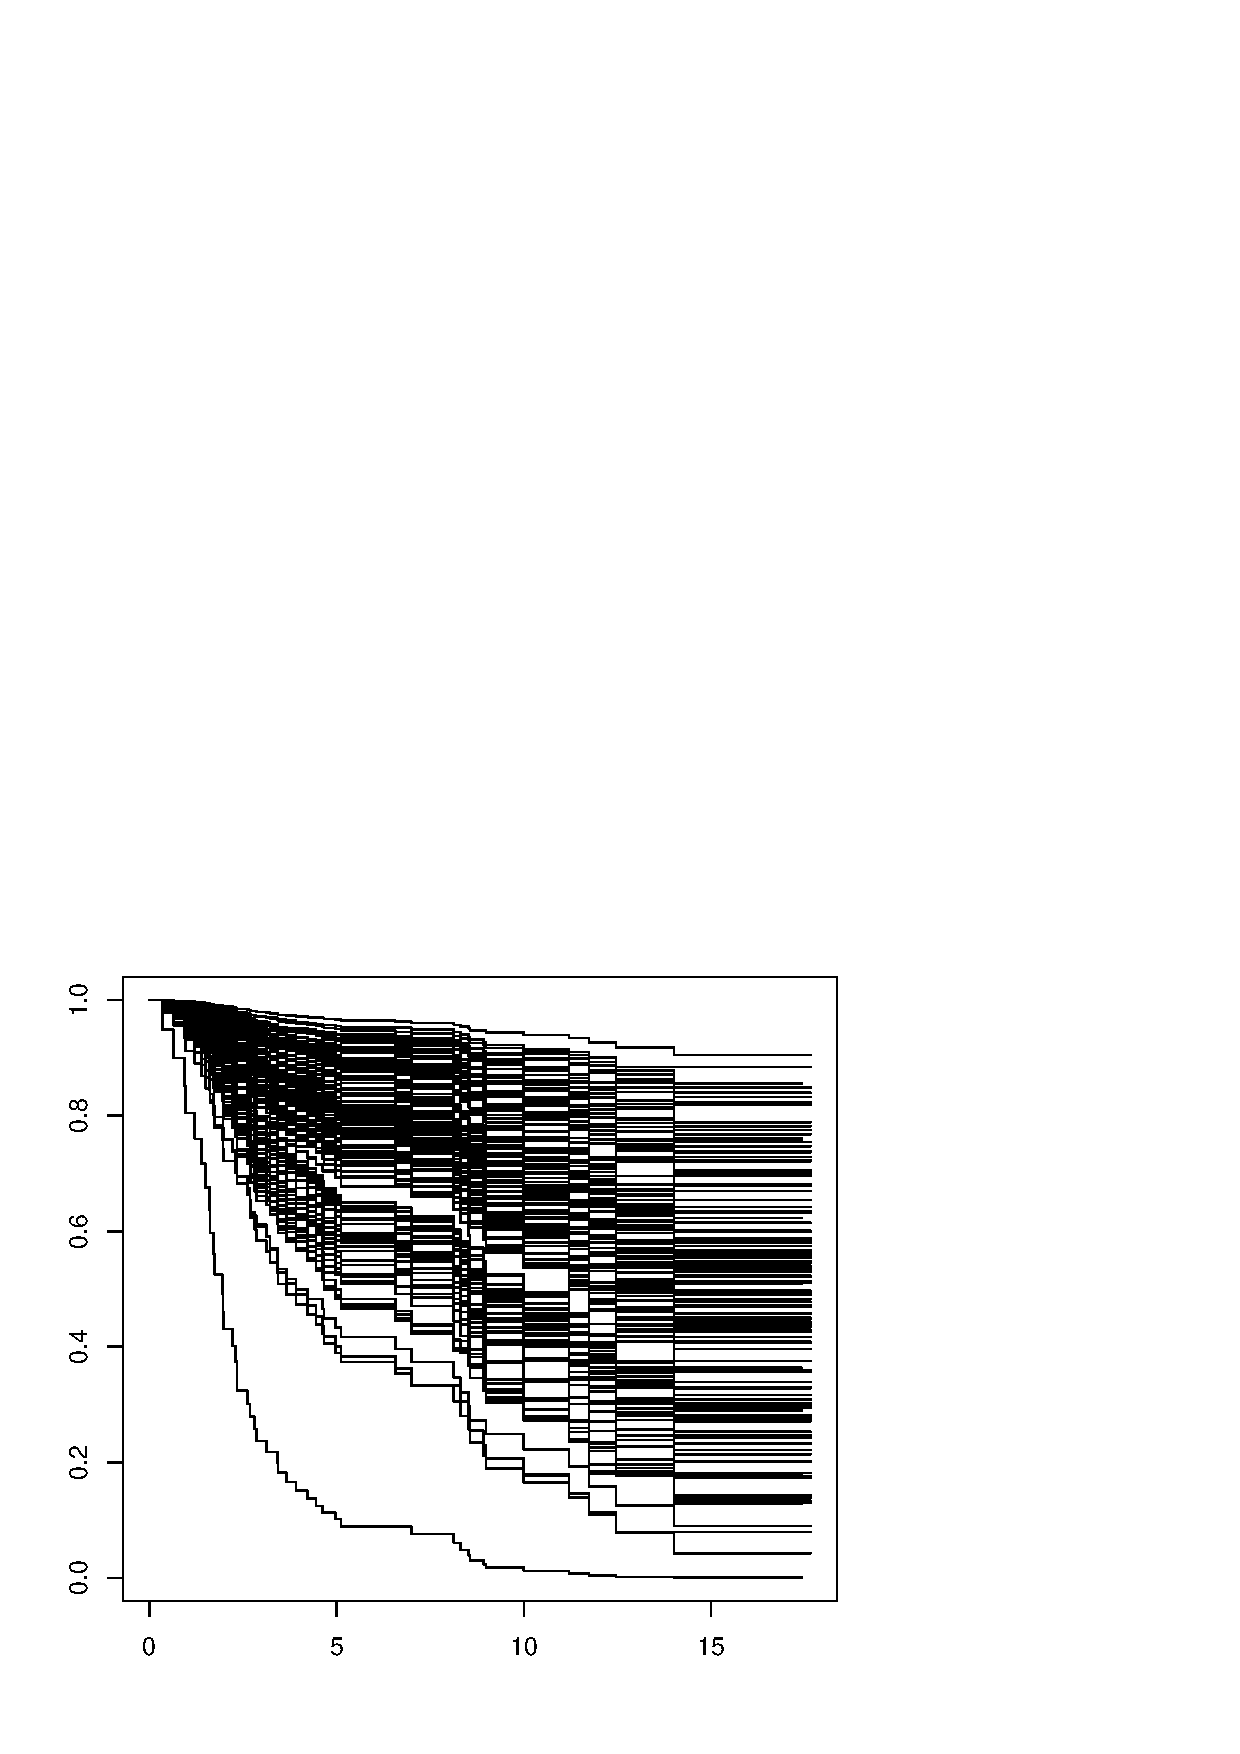
\includegraphics{penalized-breslowplot}
\end{figure}

\subsection{profiling the cross-validated log likelihood}

The functions \Rfunction{profL1} and \Rfunction{profL2} can be used to examine the effect of the parameters $\lambda_1$ and $\lambda_2$ on the cross-validated log likelihood. The \Rfunction{profL1} function can be used to vary $\lambda_1$ while keeping $\lambda_2$ fixed, vice versa for \Rfunction{profL2}.

The minimum and maximum values between which the cross-validated log likelihood is to be profiled can be given as \Rfunarg{minlambda1} and  \Rfunarg{maxlambda1} or \Rfunarg{minlambda2} and  \Rfunarg{maxlambda2}, respectively. The default value of \Rfunarg{minlambda1} and  \Rfunarg{minlambda2} is at zero.  The default value of \Rfunarg{maxlambda1} is at the maximal value of $\lambda_1$, that is the smallest value that shrinks all regression coefficients to zero. There is no default for \Rfunarg{maxlambda2}.

The number of steps between the minimal and maximal values can be given in the \Rfunarg{steps} argument (default 100). These steps are equally spaced if the argument \Rfunarg{log} is \Robject{FALSE} or equally spaced on the log scale if the argument \Rfunarg{log} is \Robject{TRUE}. Note that the default value of \Rfunarg{log} differs between \Rfunction{profL1} (\Robject{FALSE}) and \Rfunction{profL2} (\Robject{TRUE}). If \Rfunarg{log} is \Robject{TRUE}, \Rfunarg{minlambda1} or \Rfunarg{minlambda2} must be given by the user as the default value is not usable.

By default, the profiling is stopped prematurely when the cross-validated log likelihood drops below the cross-validated log likelihood of the null model with all penalized regression coefficients equal to zero. This is done because it avoids lengthy calculations at small values of $\lambda$ when the models are most likely not interesting. The automatic stopping can be controlled using the option \Rfunarg{minsteps} (default \Rfunarg{steps}/4). The algorithm only considers stopping prematurely after it has done at least \Rfunarg{minsteps} steps. Setting \Robject{minsteps=steps} cancels the automatic stopping.

The functions \Rfunction{profL1} and \Rfunction{profL2} return a named list with the same elements as returned by \Rfunction{cvl}, but each of \Robject{cvl}, \Robject{predictions}, \Robject{fullfit} is now a \Rclass{vector} or a \Rclass{list} (as appropriate) as multiple cross-validated likelihoods were calculated. An additional vector \Robject{lambda} is returned which lists the values of $\lambda_1$ or $\lambda_2$ at which the cross-validated likelihood was calculated.

The allocation of the subjects into cross-validation folds is done only once, so that all cross-validated likelihoods are calculated using the same allocation. This makes the cross-validated log likelihoods more comparable. As in \Rfunction{cvl} the allocation is returned in \Robject{fold}.

It is also possible in these functions to set \Robject{fold = 1}. This will cause no cross-validation to be performed, but will let only the full data fits be calculated. This can be used in a similar way to the use of the \Rfunction{penalized} function with its \Rfunarg{steps} argument, only with more flexibility. 

\begin{Schunk}
\begin{Sinput}
> fit1 <- profL1(Surv(time, event), nki70[, 50:70], fold = 10)
> plot(fit1$lambda, fit1$cvl, type = "l")
> fit2 <- profL2(Surv(time, event), nki70[, 50:70], fold = fit1$fold, 
      minl = 0.01, maxl = 1000)
> plot(fit2$lambda, fit2$cvl, type = "l", log = "x")
\end{Sinput}
\end{Schunk}

\begin{figure}
\begin{Schunk}
\begin{Sinput}
> plot(fit1$lambda, fit1$cvl, type = "l")
\end{Sinput}
\end{Schunk}
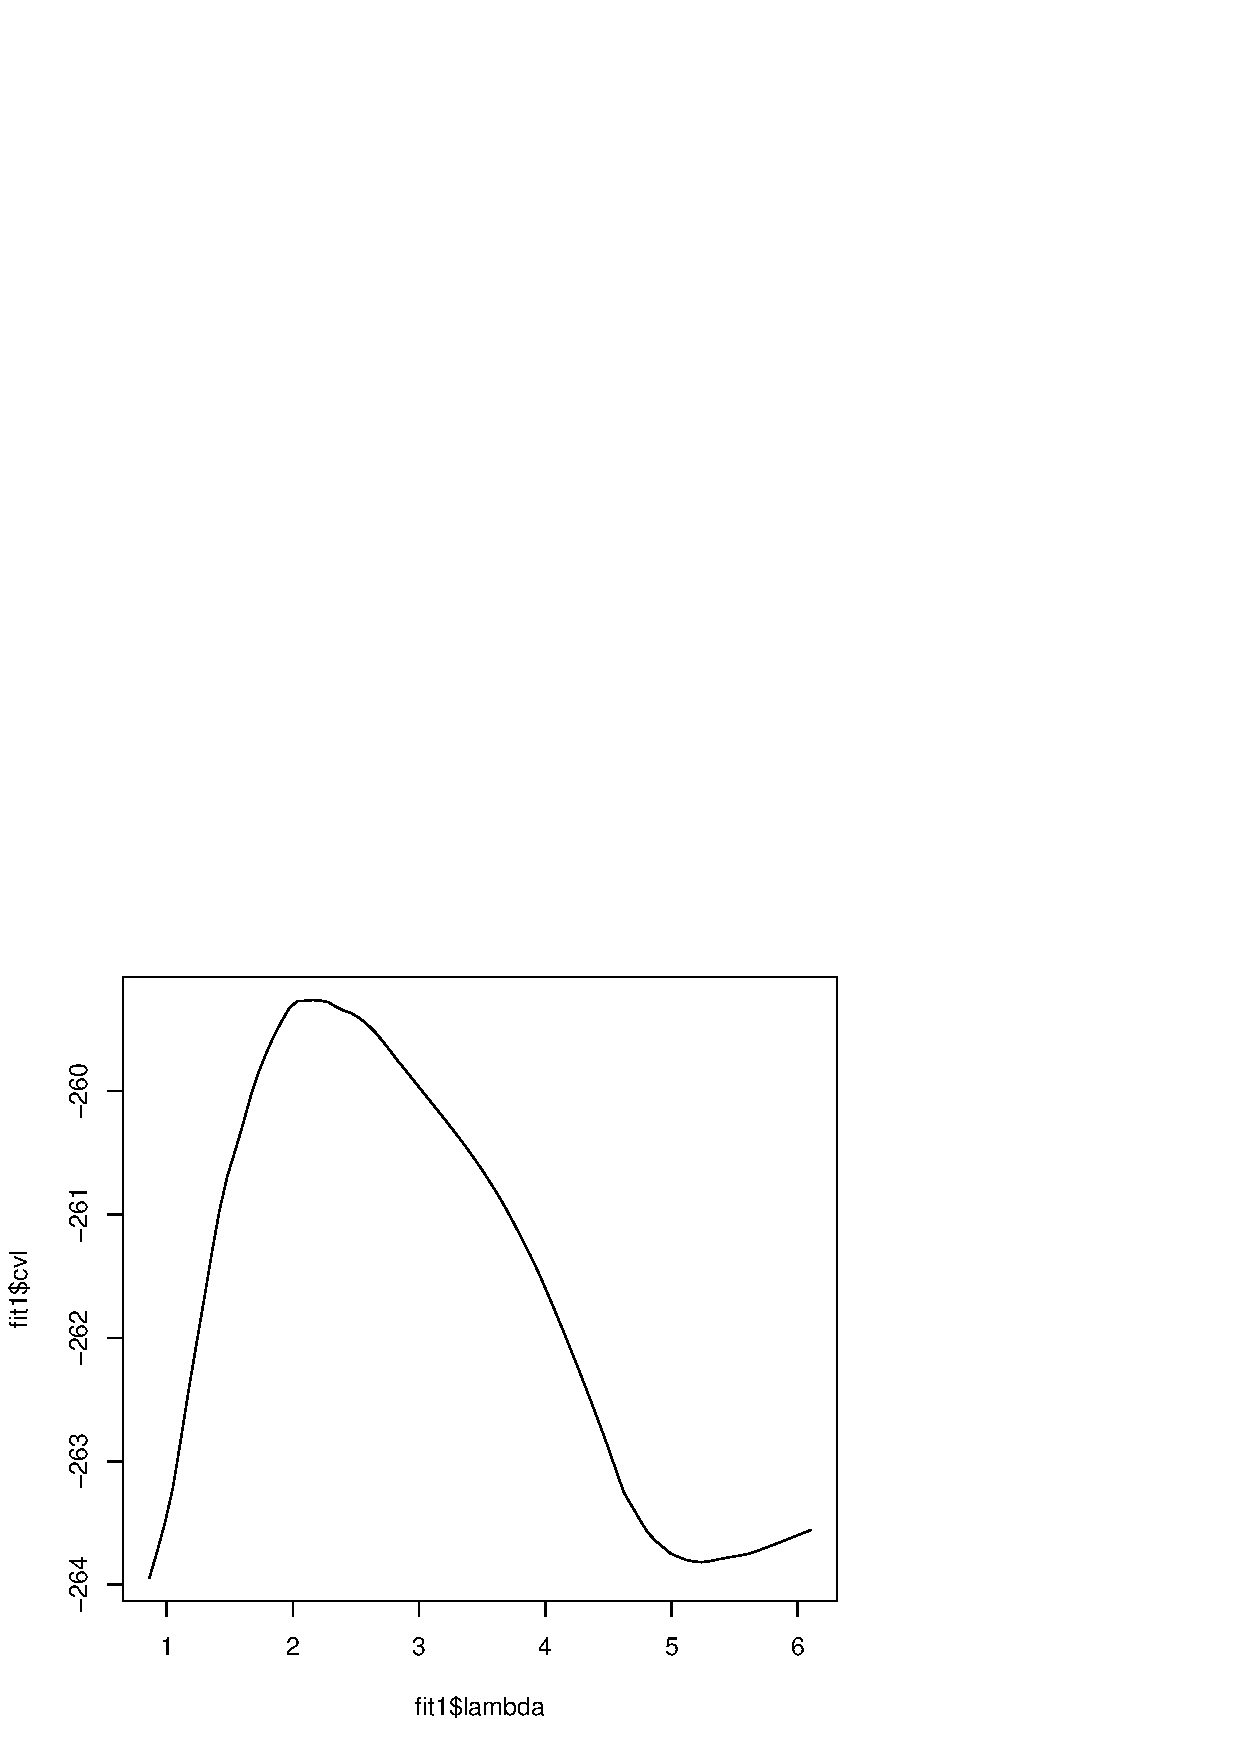
\includegraphics{penalized-profplot1}
\end{figure}

\begin{figure}
\begin{Schunk}
\begin{Sinput}
> plot(fit2$lambda, fit2$cvl, type = "l", log = "x")
\end{Sinput}
\end{Schunk}
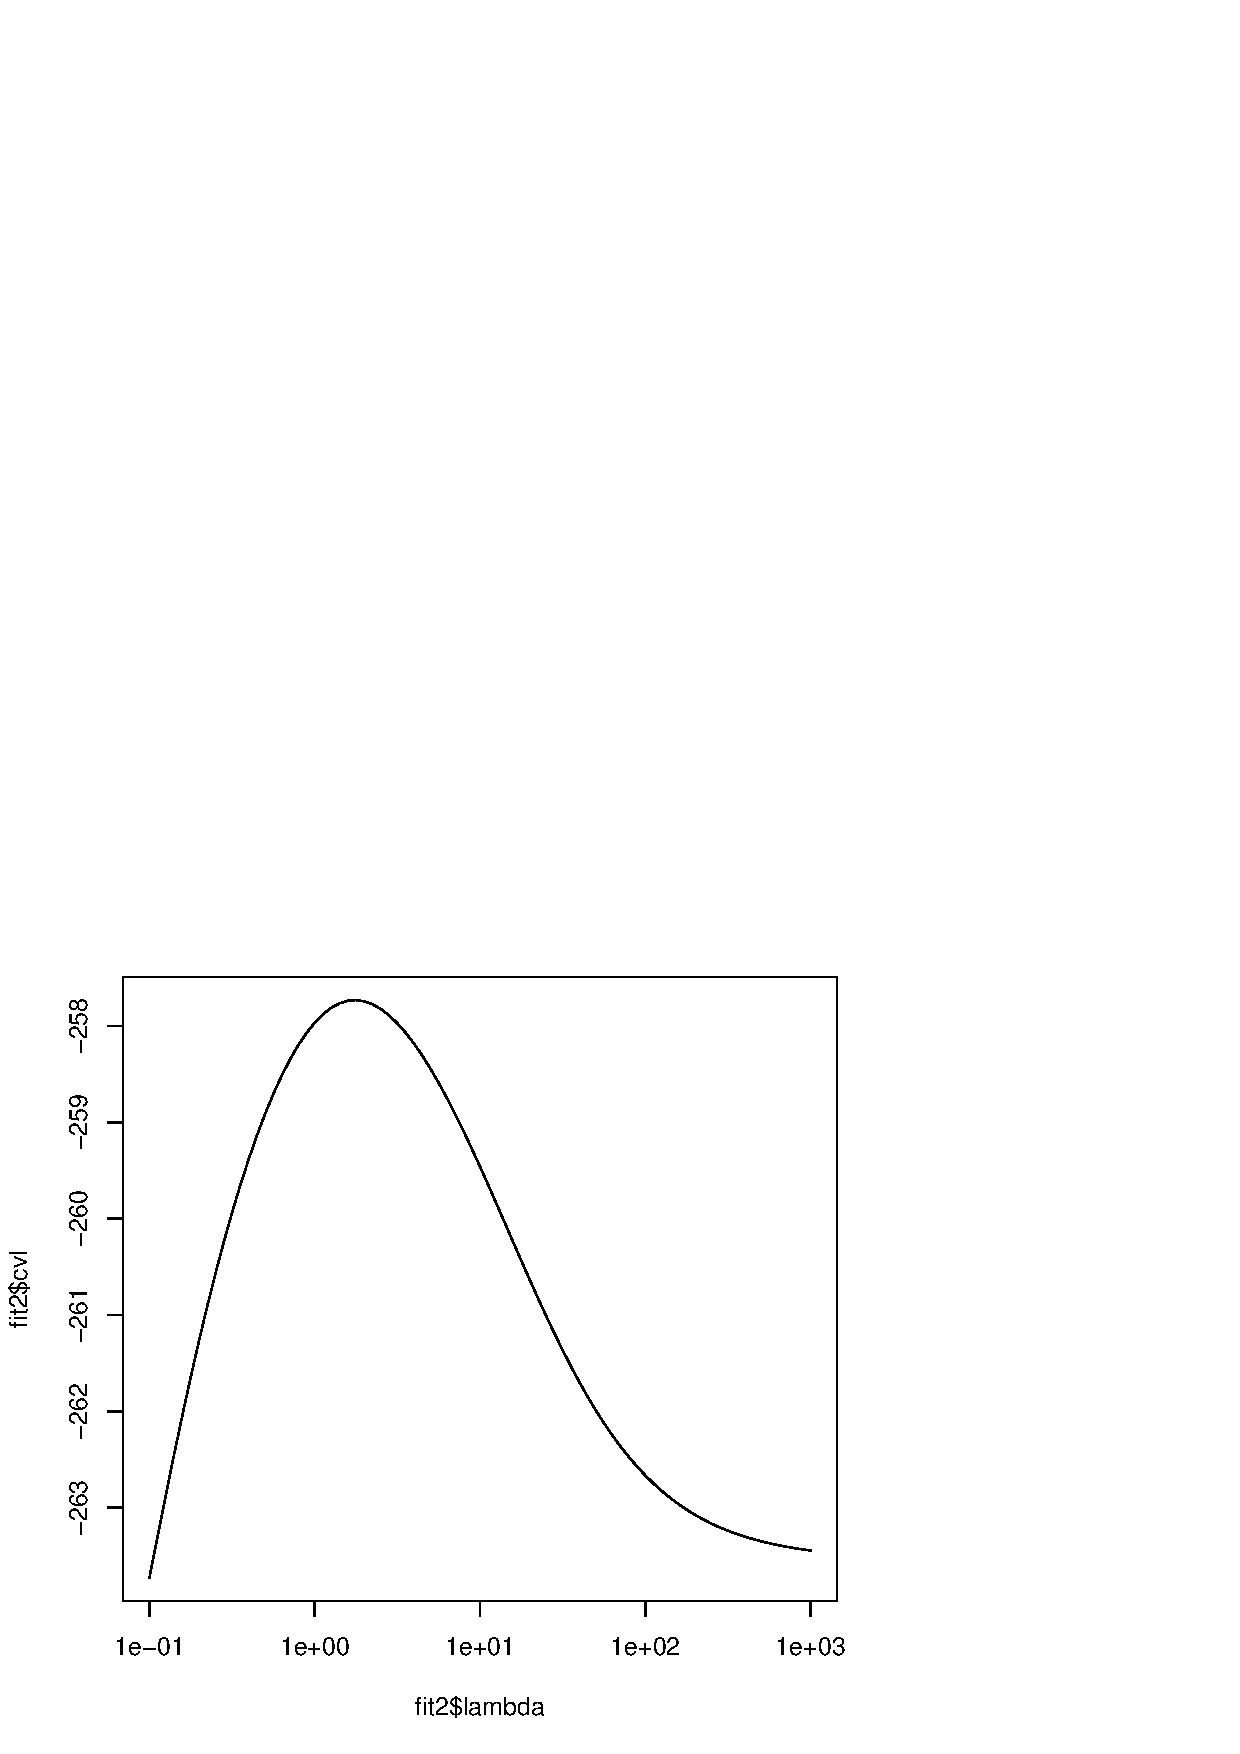
\includegraphics{penalized-profplot2}
\end{figure}

The \Rfunction{plotpath} function can again be used to visualize the effect of the tuning parameter on the regression coefficients.

\begin{Schunk}
\begin{Sinput}
> plotpath(fit2$fullfit, log = "x")
\end{Sinput}
\end{Schunk}

\begin{figure}
\begin{Schunk}
\begin{Sinput}
> plotpath(fit2$fullfit, log = "x")
\end{Sinput}
\end{Schunk}
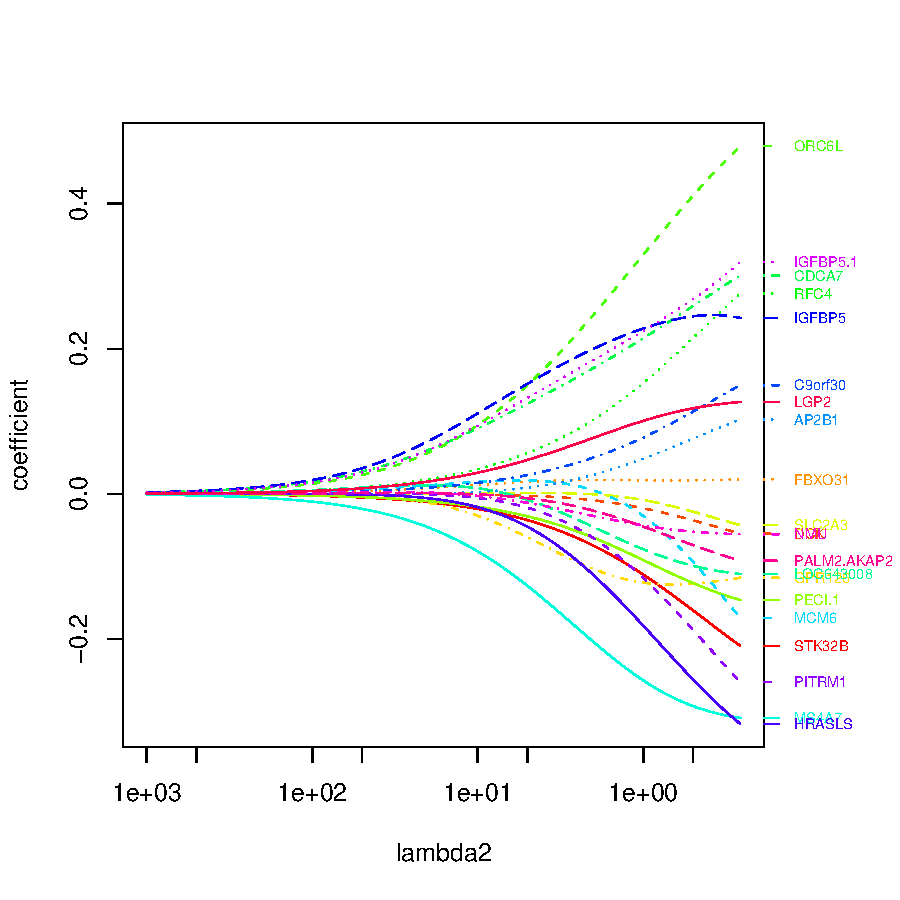
\includegraphics{penalized-profpathplot}
\end{figure}

\subsection{optimizing the cross-validated likelihood}

Often we are not interested in the whole profile of the cross-validated likelihood, but only in the optimum. The functions \Rfunction{optL1} and \Rfunction{optL2} can be used to find the optimal value of $\lambda_1$ or $\lambda_2$.

The algorithm used for the optimization is the Brent algorithm for minimization without derivatives \citep[][see also \Robject{help(optimize)}]{Brent1973}. When using this algorithm, it is important to realize that this algorithm is guaranteed to work only for unimodal functions and that it may converge to a local maximum. This is especially relevant for L1 optimization, as the cross-validated likelihood as a function of $\lambda_1$ very often has several local maxima. It is recommended to only use \Rfunction{optL1} in combination with \Rfunction{profL1} to prevent convergence to the wrong optimum. The cross-validated likelihood as a function of $\lambda_2$, on the other hand, is far better behaved and practically never has local maxima. The function \Rfunction{optL2} can safely be used even without combining it with \Rfunction{profL2}.

The functions \Rfunction{optL1} and \Rfunction{optL2} take the same arguments as \Rfunction{cvl}, and some additional ones.

The arguments \Rfunarg{minlambda1} and \Rfunarg{maxlambda1}, and \Rfunarg{minlambda2} and \Rfunarg{maxlambda2} can be used to specify the range between which the cross-validated log likelihood is to be optimized. Both arguments can be left out in both functions, but supplying them can improve convergence speed. In \Rfunction{optL1}, the parameter range can be use to ensure that the function converges to the right maximum. In \Rfunction{optL2} the user can also supply only one of \Rfunarg{minlambda2} and \Rfunarg{maxlambda2} to give the algorithm advance information of the order of magnitude of $\lambda_2$. In this case, the algorithm will search for an optimum around \Rfunarg{minlambda2} or \Rfunarg{maxlambda2}.

The functions \Rfunction{optL1} and \Rfunction{optL2} return a named list just as \Rfunction{cvl}, with an additional element \Robject{lambda} which returns the optimum found. The returned \Robject{cvl}, \Robject{predictions}, \Robject{fullfit} all relate to the optimal $\lambda$ found.

\begin{Schunk}
\begin{Sinput}
> opt1 <- optL1(Surv(time, event), nki70[, 50:70], fold = fit1$fold)
\end{Sinput}
\end{Schunk}
\begin{Schunk}
\begin{Sinput}
> opt1$lambda
\end{Sinput}
\begin{Soutput}
[1] 2.411398
\end{Soutput}
\begin{Sinput}
> opt1$cvl
\end{Sinput}
\begin{Soutput}
[1] -259.4892
\end{Soutput}
\end{Schunk}
\begin{Schunk}
\begin{Sinput}
> opt2 <- optL2(Surv(time, event), nki70[, 50:70], fold = fit2$fold)
\end{Sinput}
\end{Schunk}

\bibliography{penalized}

\end{document}


















